\documentclass{article}

\usepackage{Mathematics}
\usepackage{tabularray}
\usepackage{tikz}
\usetikzlibrary{arrows.meta}
\definecolor{flowblue}{HTML}{4F7FB7}
\pdftitle{CE-SB}

% === TITLE ===
\title{\textbf{Corporate Ethics and Sustainability \\ HSLU, Semester 5}}
\author{Matteo Frongillo}
\date{}

% === TEXT ===
\begin{document}

\maketitle
\tableofcontents
\pagebreak

\section{Introduction to Business ethics}
\subsection{Morality vs Ethics bs Ethical theory}

\begin{center}
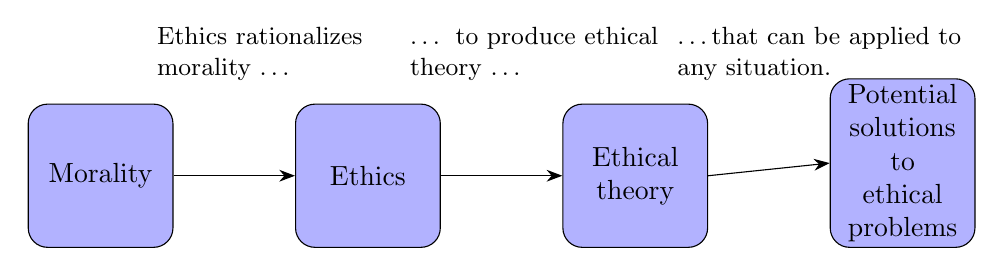
\begin{tikzpicture}[
    box/.style={draw, rounded corners=7pt, fill=blue!30,
        minimum width=.15\linewidth, minimum height=.15\linewidth,
        text width=.14\linewidth, align=center, inner sep=2pt,
        font=\normalsize},
    explanation/.style={anchor=south west, align=left, font=\small,
        inner sep=0pt},
    arrow/.style={-{Stealth[length=2mm]}, thin}
]
    \node[box, anchor=south west] (morality) at (0,0) {Morality};
    \node[box, anchor=south west] (ethics) at (.28\linewidth,0) {Ethics};
    \node[box, anchor=south west] (theory) at (.56\linewidth,0) {Ethical\\theory};
    \node[box, anchor=south west] (solutions) at (.84\linewidth,0)
        {Potential\\solutions to\\ethical\\problems};

    \draw[arrow] (morality.east) -- (ethics.west);
    \draw[arrow] (ethics.east) -- (theory.west);
    \draw[arrow] (theory.east) -- (solutions.west);

    \node[explanation] at (.135\linewidth,.175\linewidth)
        {Ethics rationalizes\\morality \ldots};
    \node[explanation] at (.40\linewidth,.175\linewidth)
        {\ldots{} to produce ethical\\theory \ldots};
    \node[explanation] at (.68\linewidth,.175\linewidth)
        {\ldots that can be applied to\\any situation.};
\end{tikzpicture}
\end{center}

\subsubsection{Morality}
Norms, values, and beliefs in social processes, which define right
and wrong for individuals and communities.

\subsubsection{Ethics}
Study of morality that focuses on explaining rules and principles that
determine right or wrong.

\subsubsection{Ethical theory}
Rules and principles are called ethical theories.

\subsection{Why is business corporate ethics important}
\begin{itemize}
    \item Power/influence of business in society (eg. lobbies, multinationals, banks)
    \item Potential to provide major contribution to society $\to$ provide employment, tax payments, solve social problems (eg. health)
    \item Malpractice can inflict enormous harm to society or environment (eg. accidents)
    \item Increasing demand from skateholders/society to act ethically
    \item Lack of business ethics education or training
    \item Businesses face trust decifit
    \item Growth of business ethics 'industry' (consultants, ethical products/services)
\end{itemize}

\subsection{Large vs small companies}
\begin{itemize}
    \item SMEs differ in their approach to business ethics:
    \begin{itemize}[label=$\to$]
        \item Lack of time and resources
        \item Less responsabilites to skateholders
    \end{itemize}
    \item Large companies have much more formalized approach to manage BE
\end{itemize}

\begin{center}
    \begingroup
    \small
    \setlength{\tabcolsep}{4pt}
    \renewcommand{\arraystretch}{1.25}
    \begin{tabularx}{\linewidth}{|>{\raggedright\arraybackslash}p{.18\linewidth}|*{4}{>{\raggedright\arraybackslash}X|}}
        \hline
        \textbf{Stakeholders} & \textbf{Large corporations} & \textbf{Small businesses} &
        \textbf{Civil society organizations} & \textbf{Public sector organizations} \\
        \hline
        \textbf{Responsible and/or accountable to} & Shareholders and other stakeholders &
        Owners & Donors and clients & General public, higher level government organizations \\
        \hline
        \textbf{Main constraints} & Shareholder orientation; size and complexity &
        Lack of resources and attention & Lack of resources and formal training &
        Inertia, lack of transparency \\
        \hline
    \end{tabularx}
    \endgroup
\end{center}

\newpage
\subsection{Globalization}
\begin{itemize}
    \item Globalization is a process which diminishes the necessity of a common and shared territorial basis for social, economic, and political activities, processes, and relations (``deterritorialization'')
    \item Globalization makes real-time social, political, economic, and cultural exchanges possible between people and organizations without the need for physical contact
\end{itemize}

Globalization was supported by two main developments:
\begin{enumerate}
    \item Technology (communication, transportation, digital financial streams)
    \item Policy (national territorial borders have been eroded)
\end{enumerate}

\subsubsection{Effects}
\begin{itemize}
    \item European financial crisis $\to$ events, which have local roots, have effects on seemingly disconnected places
    \item Global climate change $\to$ Local causes leads to global problems and global solutions (eg. Kyoto Protocol)
    \item Acts of Terror $\to$ events, people or ideas from faraway places can have effects on people on unconnected locations/situations (eg. security checks in airports)
\end{itemize}

\subsubsection{Ethics in the context of globalization}
\begin{itemize}
    \item Topics like fair trade, food prices, financialstability have set ethical spotlight on globalization process
    \item MNCs (Multi-National Corporations) are at the center of public's criticism on globalization\\$\to$ accused to exploit workers, cause environmental destruction,abuse their economic power
    \item Globalization is the most demanding area for corporation to define and legitimate their ``right and wrong'' behavior
\end{itemize}

\subsection{Concepts distinct from globalization}
\subsubsection{Internationalization}
Internationalization is the expansion of activities across national borders while those activities remain anchored in particular countries.

\subsubsection{Westernization}
Westernization is the spread or adoption of Western cultural practices, values, and institutions.

\subsubsection{Homogenisation}
Homogenisation is the process by which cultures, products, or practices become more similar to one another.

\subsection{Relevance of globalization for business ethics}
\subsubsection{Cultural issues}
\begin{itemize}
    \item Corporations increasingly engage in overseas markets
    \item Confronted with new, diverse or even contradictory ethical demands
\end{itemize}

\subsubsection{Legal issues}
\begin{itemize}
    \item Linked to relationship between ethics and law
    \item Transactions lose connection to certain territorial entity
    \item Escape legal control of national governments
    \item Globalization increases demand for business ethics (beyond control of national governments)
\end{itemize}

\subsubsection{Accountability issues}
\begin{itemize}
    \item Some MNCs are as economically powerful as entire countries
    \item How to control MNCs, which have higher revenues than GDPs of entire countries?
    \item Demand for corporate accountability
\end{itemize}

\begin{tblr}{
  width=\linewidth,
  colspec={|l|X[l]|},
  hlines,
  rows={valign=m, rowsep=6pt}
}
    \textbf{Stakeholders} & \textbf{Ethical impacts of globalization} \\
    Shareholders & Globalization provides potential for greater profitability, but also greater risks (e.g. financial instability). \\
    Employees & Provides jobs but also raises the potential for exploitation of employees through poor working conditions. \\
    Consumers & Global products provide social benefits to consumers across the globe, but may also meet protests about cultural imperialism and westernization. Globalization can bring cheaper prices to customers. \\
    \makecell[l]{Suppliers \&\\competitors} & Suppliers in developing countries face regulation from MNCs through supply chain management. Small-scale indigenous competitors are exposed to global players. \\
    \makecell[l]{Civil society\\(NGOs, etc.)} & Globally active pressure groups emerge with the aim to ``police'' corporations where governments are weak. \\
    ... & ... \\
\end{tblr}

\subsubsection{International differences in approaches}
\begin{tblr}{
  width=\linewidth,
  colspec={|X[2,l]|X[l]|X[l]|X[l]|},
  hlines,
  rows={valign=m, rowsep=5pt},
  row{1}={font=\bfseries},
  column{1}={font=\bfseries}
}
    & Europe & N. America & Asia \\
    Who is responsible for ethical conduct in business?
    & Social control by the collective & The individual & Top management\\
    Who is the key actor in business ethics?
    & Government, trade, unions, corporate associations & The corporation & Government, corporations\\
    What are the key guidelines for ethical behaviour?
    & Negotiated legal framework of business & Corporate codes of ethics & Managerial discretion\\
    What are the key issues in business ethics?
    & Social issues in organizing framework of business & Misconduct and immorality in single decisions situations & Accountability\\
\end{tblr}











\end{document}
